\documentclass[ %
    11pt, %
    a4paper, %
    BCOR=12mm, %
    DIV=12, %
    headsepline=true, %
    parskip=half, %
    %draft=true, %
]{article}

\usepackage[utf8]{inputenc}
\usepackage[T1]{fontenc}
\usepackage{lmodern}
%%englisches Protokoll
%\usepackage[british,UKenglish,USenglish,english,american]{babel}
% %
%%deutsches Protokoll
\usepackage[ngerman]{babel}
% %
\usepackage{amssymb,amsmath}
\usepackage{engrec}
\usepackage{enumerate}
\usepackage{empheq}
\usepackage{picins}
\usepackage{floatflt}
\usepackage{graphicx}
\usepackage{color}
\usepackage{natbib}
\usepackage{pdfpages}
\usepackage{hyperref}
\graphicspath{{Bilder/}}%% Allgemeine Bilder
\usepackage[paper=a4paper,left=25mm,right=25mm,top=25mm,bottom=25mm]{geometry}

\begin{document}


\begin{titlepage}

\begin{center}




\includegraphics[width=0.3\textwidth]{Bilder/logo}\\[1.2cm]    

\textsc{\LARGE Albert-Ludwigs-Universit\"at Freiburg}\\[1.75cm]

\textsc{\Large Physikalisches Fortgeschrittenen-Praktikum I}\\[0.75cm]



\newcommand{\HRule}{\rule{\linewidth}{0.5mm}}
\HRule \\[0.5cm]
{ \huge \bfseries Szintillationszähler}\\[0.5cm]

\HRule \\[1.75cm]


\begin{minipage}{0.4\textwidth}
\begin{flushleft} \large
\emph{Studenten:}\\
Daniel \textsc{Uhl}\\ \setlength{\parindent}{1.25cm} \& 
\setlength{\parindent}{0cm} \\ Jan P\'eter \textsc{Szabados} 
\end{flushleft}
\end{minipage}
\hfill
\begin{minipage}{0.4\textwidth}
\begin{flushright} \large
\emph{Tutor:} \\
Matthias \textsc{Gorzellik}\\
\end{flushright}
\end{minipage}

\vfill


{\large \today}

\end{center}

\end{titlepage}

\tableofcontents
\newpage
\newpage
\section{Ziel des Versuchs}
Bei bestimmten Materialen kann man beim Anlegen eines elektrischen oder magnetischen Feldes Doppelbrechung beobachten. Im Falle des elektrischen Feldes spricht man von elektrooptischen Effekt und unterscheidet hier zwischen einer linearen (Pockels) und einer quadratischen (Kerr) Abhängigkeit. Im zweiten Fall spricht man vom magnetooptischen oder Faraday-Effekt. Ziel des Versuches ist es das Tensorelements, welches die Brechung in Ammoniumdihydrogenphosphat (ADP) beschreibt beim Pockelseffekt und die Verdetkonstante von Schwerflintglas mit dem Faraday-Effekt zu bestimmen.
~\\
~\\
~\\
~\\
~\\
~\\
\section{Aufgabenstellung}
\begin{itemize}
\item Mit der Hilfe des Pockels-Effekts wird der elektrooptische Koeffizient $r_{41}$ von ADP bestimmt. Die zur Berechnung benötigte Halbwellenspannung wird hierfür auf zwei verschieden Arten bestimmt:
\begin{itemize}
\item Sägezahnmethode
\item Modulierte Gleichspannung
\end{itemize}
\item Bestimmung der Verdetkonstante von Schwerflintglas bei Licht einer Wellenlänge von $\lambda = 589 nm $ mithilfe des Faraday-Effekts, indem der Ablenkwinkel bei unterschiedlicher Magnetfeldstärke, von linear polarisiertem Licht, gemessen wird.
\end{itemize}
\clearpage
\section{Theoretische Grundlagen}
\subsection{Doppelbrechung}
Es existieren Materialien in denen die Lichtgeschwindigkeit $v$ in alle Richtungen gleich ist und Materialien in welchen die Lichtgeschwindigkeit für verschiedene Richtungen verschiedene charakteristische Werte aufweist. Im ersten genannten Fall spricht man von einem optisch isotropen Medium, im zweiten von einem optische anisotropen Medium.\\
In einem optisch isotropen Medium gib es somit einen Brechungsindex n welcher durch den Quotienten aus $c$ und $v$. Bei optisch anisotropen Materialien geht diese skalare Größe in einen Tensor $n_{ij}$ mit $i,j = 1, ...,3$ über. Um nun die Ausbreitungsgeschwindigkeit einer linear polarisierten Welle zu beschreiben, führt man das Indexellipsoid ein, welches gegeben ist durch:
\[ \sum\limits_{i,j=1}^{3} B_{ij} x_j x_i = 1 ~~,~~ wobei ~ B_{ij}=\frac{1}{n_{ij}^2} .\]

\begin{floatingfigure}[l]{5.5cm}
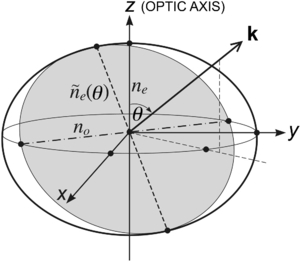
\includegraphics[scale=1.5]{ellipso}
\caption{Ellipsoid zum Bestimmen der charakteristischen Lichtgeschwindigkeit, Quelle: [iop]}
\label{fig:ellipso}
\end{floatingfigure}

Eine senkrecht zur Ausbreitungsrichtung der Lichtwelle stehende Ebene schneidet das Indexellipsoid auf einer Ellipse. Die Längen der Halbachsen geben die Größe des Brechungsindex an, für eine Lichtwelle welche in entlang der Halbachse linear polarisiert ist. Da wir jede Lichtwelle durch eine Superposition aus zwei entlang der Halbachsen polarisierten Wellen beschreiben können, erhalten wir zwei mit unterschiedlicher Geschwindigkeit ausbreitende Wellen. Dies nennt man Doppelbrechung.
~\\
~\\
\subsection{Pockels-Effekt/ Linearer elektrooptischer Effekt}
Der Pockels-Effekt ist auf der Tatsache begründet, dass die Permittivität $\epsilon=\frac{\partial D}{\partial E}$ nicht konstant ist, sondern vom elektrischen Feld abhängt. Das bedeutet, dass D nicht rein linear von E abhängt, sodass gilt: $\epsilon=a+2bE+3cE^{2}+...$. Da der Brechungsindex von der Permittivität abhängt, bedeuten Anderungen in $\epsilon$ auch Anderungen in diesem. Andert sich der Brechungsindex eines Kristalls durch ein äußeres elektrisches Feld, so spricht man vom elektrooptischen Effekt. Der lineare Anteil in der Formel $2bE$ bewirkt den Pockels-Effekt.\\
\begin{floatingfigure}[l]{11cm}
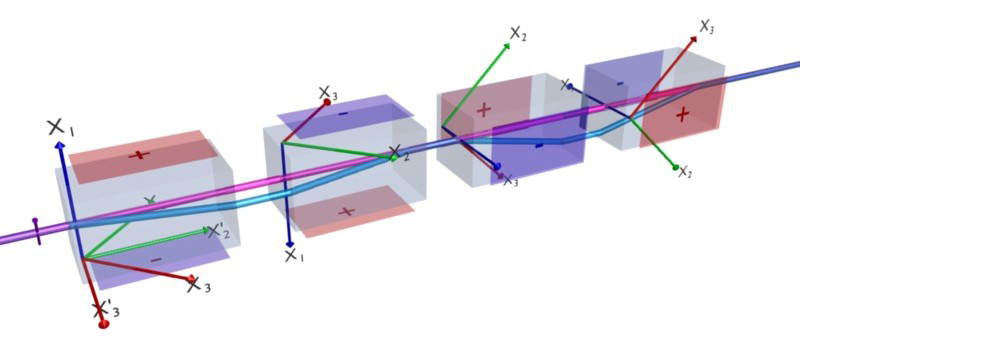
\includegraphics[scale=0.4]{aufbaupock.png}
\caption{Pockels-Zelle; Quelle: [ver]}
\end{floatingfigure}
Um kleine Veränderungen von $\epsilon$ und somit im Brechungsindex n messen zu können, kann die Doppelbrechung ausgenutzt werden. Andert sich der Brechnungsindex, so wird der Indexellipsoid umgeformt. In diesem Versuch werden Kristalle verwendet, in welchen nur der lineare elektrooptische Effekt, also der Pockels-Effekt, von Bedeutung ist. Diese sind in einem $45\,^{\circ}-Y-Cut$ (s. [Ver]) angeordnet. Mit dem Versuch messen wir die Halbwellenspannung $U_{\lambda/2}$: Für eine "Pockels-Zelle" ist das diejenige Spannung, die eine Phasenverschiebung von $\pi$ induziert.\\

Die Pockels-Zelle, welche wir verwenden, ist aus vier Kristallen aufgebaut. Die Anzahl ist wegen der Doppelbrechung so festgesetzt: Die zwei Kristallpaare bestehen aus jeweils zwei Kristallen derselben Orientierung. Die Paare sind zueinander um $90\,^{\circ}$ verschoben. Dieser Aufbau bewirkt folgendes: Das eintreffende Licht erreicht den ersten Kristall und wird aufgespalten. Der nächste Kristall macht diese Aufspaltung rückgängig. Um die natürliche Phasenverschiebung auszugleichen (damit nur die durch den Pockels-Effekt verursachte Verschiebung übrig bleibt), wird das zweite Kristallpaar gebraucht: Der dritte Kristall hat nämlich eine um $90\,^{\circ}$ verschobene Orientierung. Da das Licht aber wieder aufgespalten wird, benötigt man den 4. Kristall, um diesen Effekt rückgängig zu machen.
\subsection{Magnetooptischer Effekt/ Faraday-Effekt}
Passiert linear polarisiertes Licht längs eines homogenen Magnetfeldes ein Medium, so kann man beobachten, dass sich die Polarisierungsebene verdreht. Der Drehwinkel ist proportional zur magnetischen Feldstärke $H$ und zur Länge $l$ welche das Licht im Material zurücklegt. Wir erhalten somit:
\[ \alpha = V \cdot H \cdot l \]
Der Proportionalitätsfaktor $V$ ist nicht von $H$ oder $l$ abhängig. $V$ wird Verdetkonstante genannt und ist abhängig vom Material des Mediums und der Wellenlänge des Lichts.
\subsection{Halbschattenpolarimeter}
Ein Halbschattenpolarimeter ist ein Aufbau aus eine Polarisator, einem Analysator und einem Prisma. Nach dem Polarisator rotiert ein Prisma einen Teilbereich des einfallenden Lichtes, so dass zwei Lichstrahlen mit einem Polarisationsunterschied von einem Winkel $\epsilon$ entsteht. Zwischen Prisma und Analysator wird eine Probe platziert. Am Analysator kann man nun zwei verschieden helle Flächen sehen. Um nun herauszufinden wie die Probe die Polarisationsebene gedreht hat muss man den Analysator so drehen das nur noch eine gleich helle Fläche zu sehen ist.
\newpage
\section{Durchführung}
\subsection{Pockels-Effekt}
\begin{figure}[h]
\begin{center}
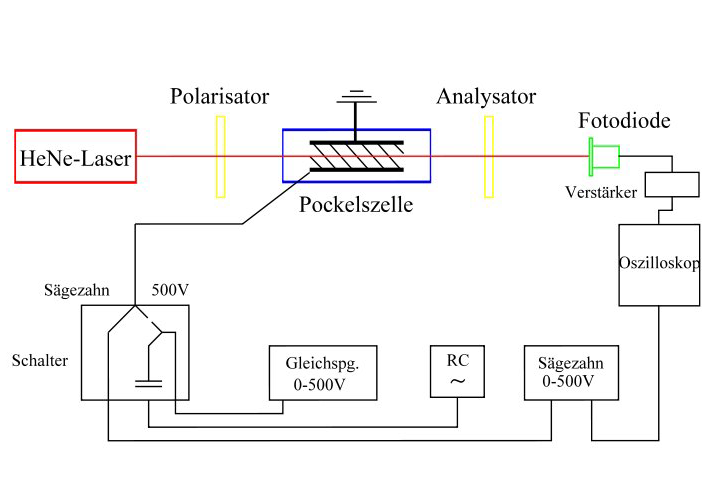
\includegraphics[scale=0.5]{durchpock.png}
\caption{Aufbau}
\end{center}
\end{figure}
Der Aufbau besteht aus einem He-Ne-Laser als Lichtquelle, welche ihren Strahl durch einen Polarisator sendet, der dafür sorgt, dass das Licht linear polarisiert ist. Nach diesem Vorgang trifft der Strahl auf die Pockels-Zelle, in welcher die Richtung der Polarisation verändert wird. Zunächst ist dieser Aufbau zu justieren. Ein Analysator wird verwendet, um die Intensität abhängig von dem Winkel relativ zur Polarisationsrichtung zu verändern. Das Licht wird schließlich von einer Photodiode mit einem Verstärker detektiert. Das nachgeschaltete Oszilloskop stellt den Verlauf des resultierenden Signals dar. Es kann auch das Eingangssignal anzeigen. Die unterschiedlichen Spannungsverläufe werden von einem Spannungsgenerator geliefert. Die auf dem Oszilloskop dargestellten Signale können mithilfe eines Computerprogramms ausgelesen werden. Es ist darauf zu achten, dass die Auflösung auf dem Oszilloskop möglich groß ist und die Signale komplett auf den Bildschirm passen. Damit nehmen wir dann mithilfe des PC-Programmes den Kurvenverlauf auf und schließlich auch ein gedämpftes und ein ungedämpftes Signal. Im zweiten Teil des Versuchs (für den Sinus-Verlauf) muss am Spannungsgenerator die Spannung verändert werden, bis eine Verdopplung der Frequenz beobachtet wird. Diese Messreihe wird für negative wie positive Spannungen öfters wiederholt.

\subsection{Faraday-Effekt}
\begin{figure}[h]
\begin{center}
\includegraphics[scale=0.3]{auf_fara}
\caption{Versuchsaufbau zum Faraday-Effekt; (1)Wasserkühlung, (2)Spule mit Schwerflintstab, (3)Na-Lampe, (4)Analysator des Halbschattenpolarimeters, (5)Okular; Quelle: [ver]}
\label{fig:auf_fara}
\end{center}
\end{figure}
\begin{floatingfigure}[l]{8.0cm}
\begin{center}
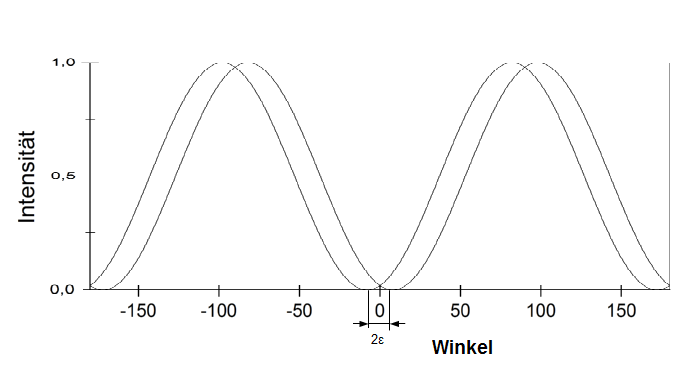
\includegraphics[scale=0.27]{2epsilon2}
\caption{Theoretische Intensität der beiden vom Halbschattenpolarimeter erzeugten Flächen.}
\label{fig:2epsilon}
\end{center}
\end{floatingfigure}
 Der Aufbau ist wie in Abbildung \ref{fig:auf_fara} gegenben. Einige Minuten vor Beginn der Versuchsdurchführung wird die Wasserkühlen der Spule und die Natriumdampflampe angeschaltet. Um später den Ablesefehler besser abschätzen zu können wurden hier zu beginn mehrere Messwerte aufgenommen für den Ablenkwinkel bei einem Spulenstrom von $I=0A$. Dabei das Halbschattenpolarimeter mehrmals von der Ausgleichslage (Position bei der die Felder gleich hell sind) weg gedreht und frisch eingestellt.
Nun wurden die Winkel für verschieden Stromstärken gemessen, es wird in $0,5A$ Schritten von etwa $-4,5A$ bis $+4,5A$ gemessen. Dabei wird der Winkel in der Ausgleichslage zur jeweiligen Stromstärke notiert.\\
Um den $2 \epsilon$-Winkel, der Winkel um welchen die Hälften zueinander verschoben sind,zu bestimmen, muss einmal der Winkel gemessen werden bei dem die (hier) äußeren Flächen am dunkelsten sind und die innere Fläche am hellsten und den Winkel bei der inversen Helligkeitsauflösung. Der $2 \epsilon$-Winkel ist dabei die Differenz der beiden gemessenen Winkel.

\clearpage
\section{Auswertung}
\subsection{Pockels-Effekt}
Um den elektrooptischen Koeffizienten $r_{41}$ von ADP berechnen zu können, benutzten wir zwei verschiedene Methoden, um die Spannung $U_{\lambda/2}$, welche die Polarisation des einfallenden Lichtes um $90\,^{\circ}$ dreht.\\
\subsubsection{Sägezahnmethode}
Wir benutzten einen Spannungsgenerator, welcher ein Sägezahnsignal mit der Frequenz $\nu=30 Hz$ generiert. Die Spannung steigt daher konstant an. Dies bewirkt ein sinusförmiges Signal an der Fotodiode. \\
\begin{figure}[h]
\begin{center}
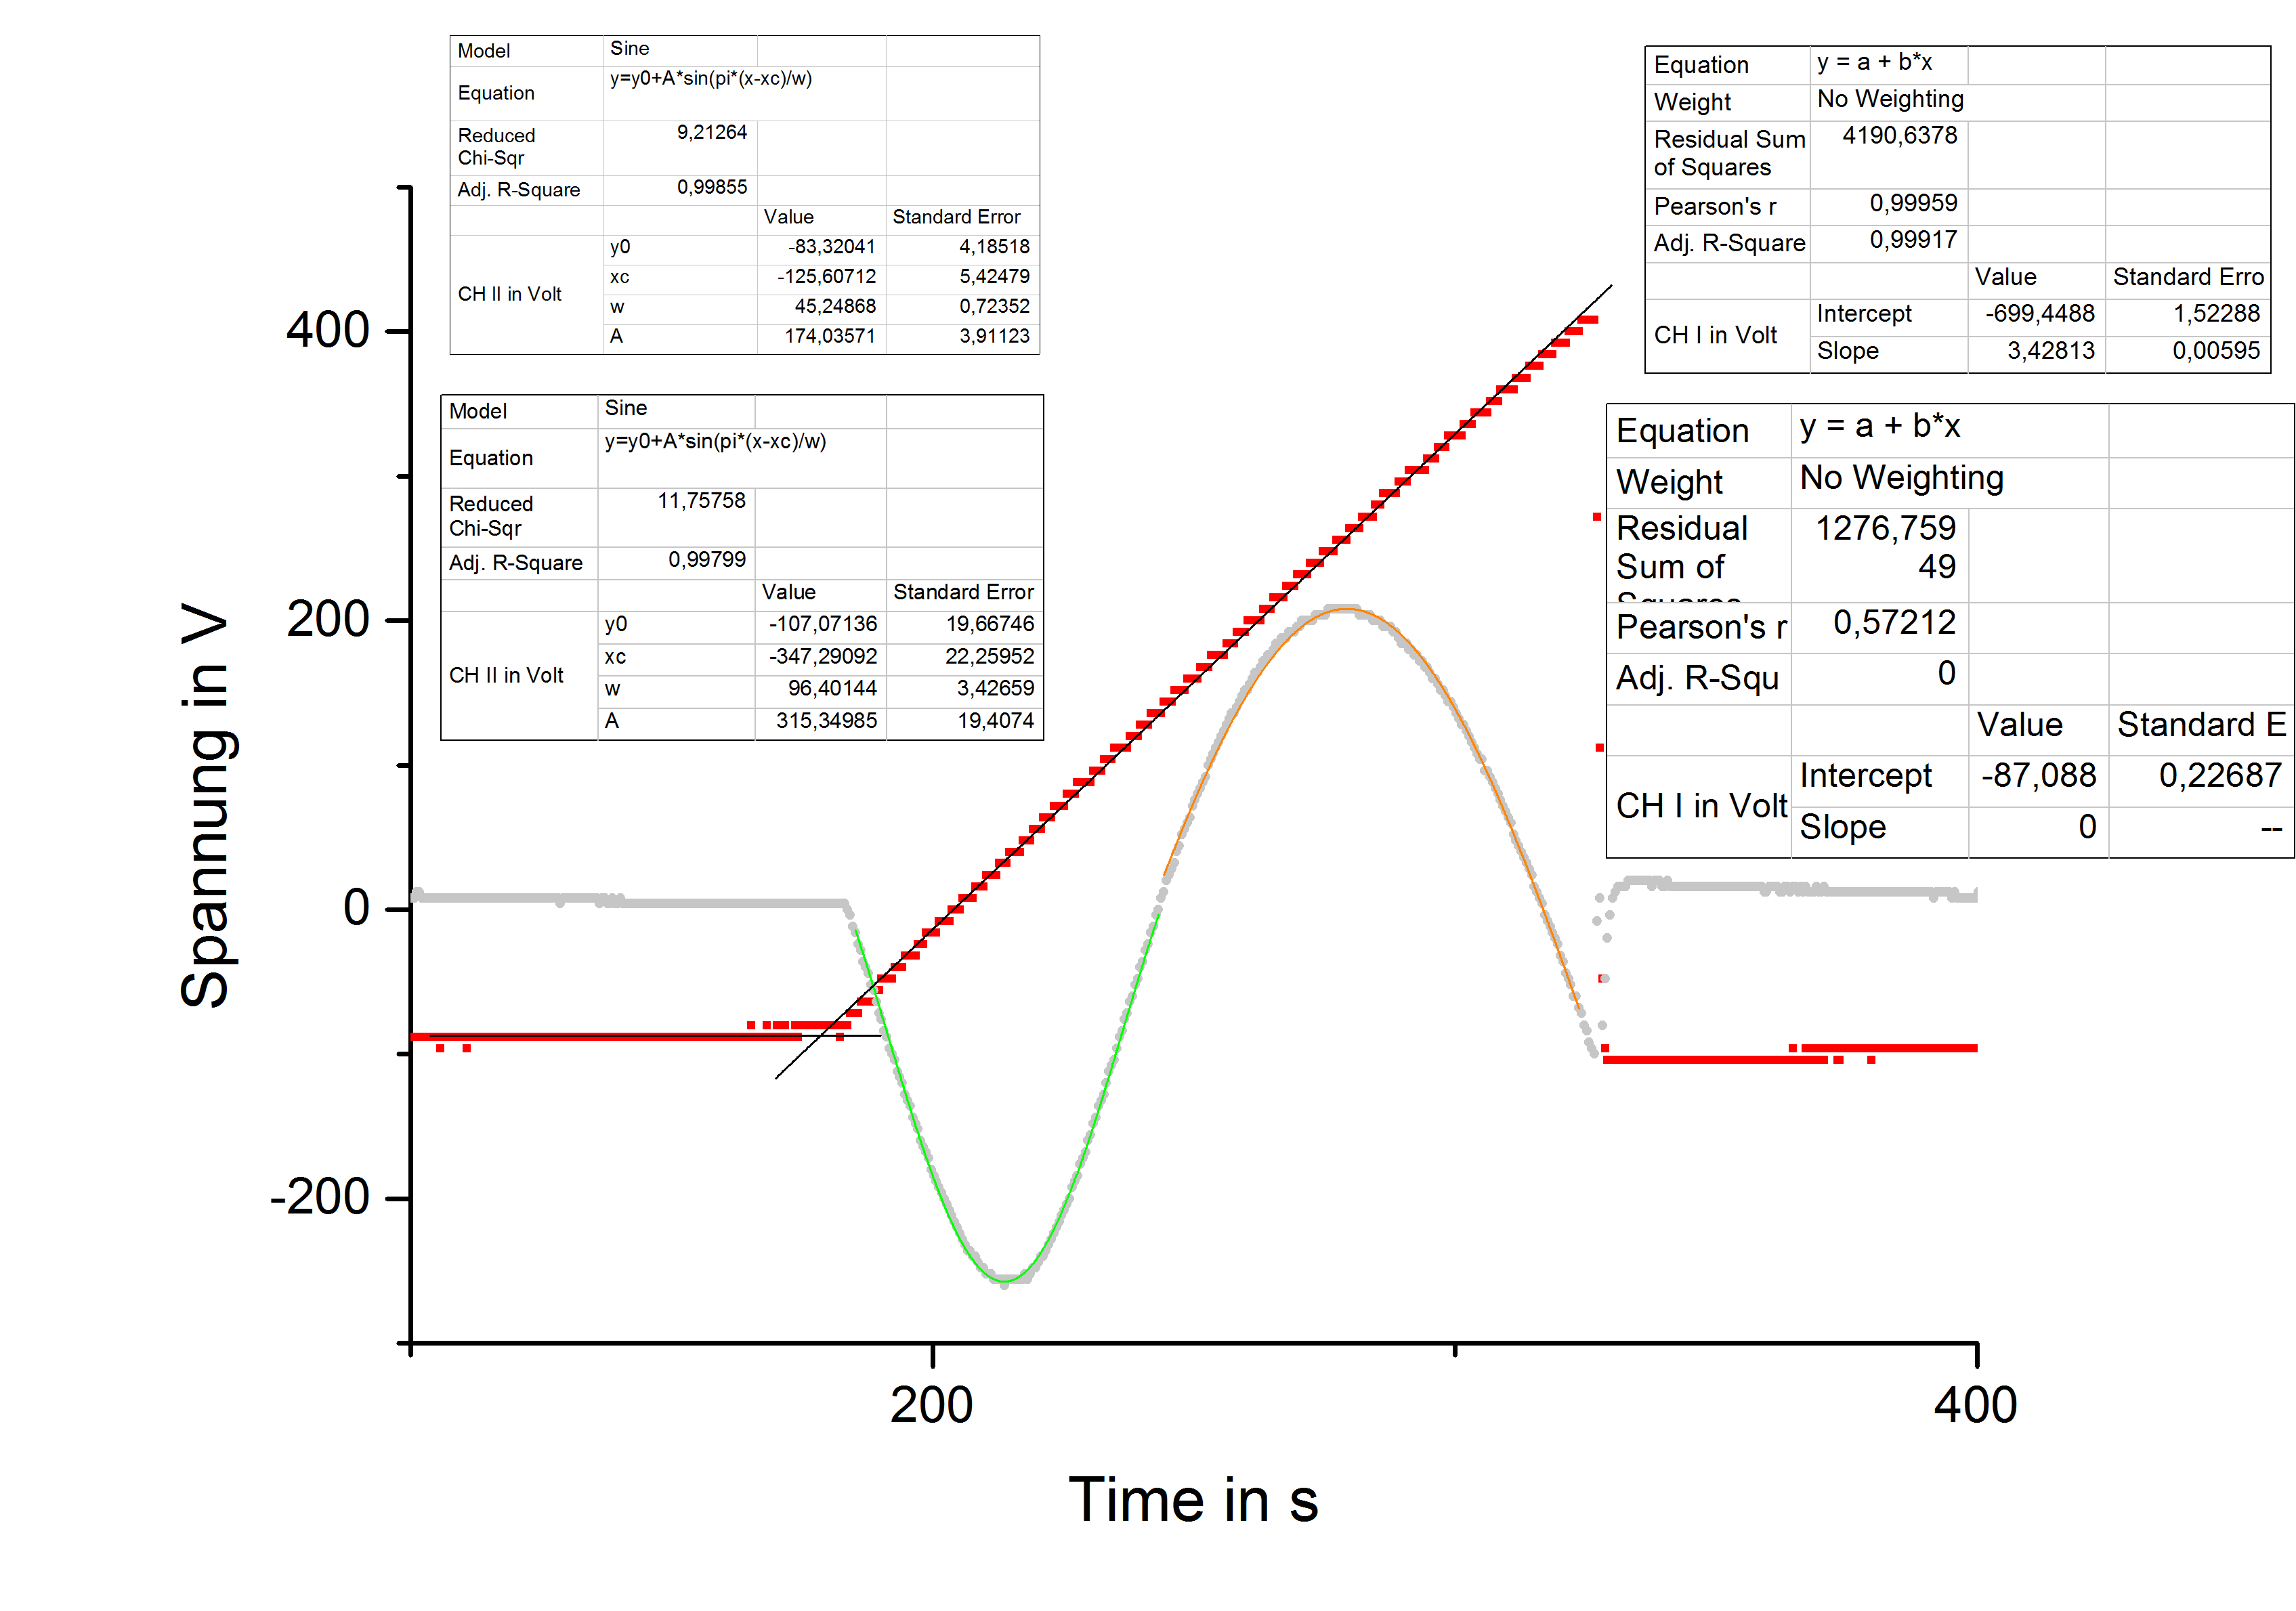
\includegraphics[scale=0.6]{anpassung1.png}
\caption{Durch Sägezahnspannung erzeugtes Signal}
\end{center}
\end{figure}
\clearpage
Wir entschlossen uns, an den negativen wie den positiven Peak des Signals der Fotodiode eine Sinuskurve zu fitten und mithilfe dieser die Zeiten zu bestimmen, zu welchen sie auftreten. Mithilfe der Differenz der zugehörigen Spannungen, welche zu den so bestimmten Zeiten bei dem Sägezahnsignal auftreten, lässt sich $U_{\lambda/2}$ bis auf einen Korrekturfaktor bestimmen. \\
Die Sinus-Fits haben die Form \[y=y_{0}+A*\sin(\pi*\frac{(x-x_{c})}{w})\]. Tiefpunkte erhält man dabei bei \[\frac{x-x_{c}}{w}=\frac{4k-1}{2}\], wobei $k\in \mathbb{Z}$ gilt. Analog gilt für Hochpunkte: \[\frac{x-x_{c}}{w}=\frac{4k-3}{2}\]. Für die Fehler folgt somit, wenn man nach x auflöst und die Gauss'sche Fehlerfortpflanzung verwendet: \[s_{x_{tief}}=\sqrt{(\frac{4k-1}{2})^{2}*(s_{w})^{2}+(s_{x_{c}})^{2}}\] und \[s_{x_{tief}}=\sqrt{(\frac{4k-3}{2})^{2}*(s_{w})^{2}+(s_{x_{c}})^{2}}\]. Der Fehler ist also am geringsten für $k_{tief}=0$ und $k_{hoch}=1$. Wie man bei der Betrachtung der Zeiten, zu welchen die Peaks etwa auftreten, jedoch sieht, gilt für unsere Fits $k_{tief}=4$ und $k_{hoch}=3$. Dies liegt am Auswerteprogramm Origin, welches wir verwendeten und welches die Fits auf diese Art erstellte. Um etwas kleinere Fehler zu erhalten, beschlossen wir, die Anfangszeit des Signals als Startpunkt festzusetzen. Aus diesem Grund berechneten wir den Schnittpunkt von linearem Fit der ansteigenden Sägezahnspannung und dem flachen, konstanten Bereich desselben Kanals zuvor (s. Diagramm). Somit erhielten wir für die Anfangszeit:\\
\[m*x+c=d\]
\[\Leftrightarrow x=\frac{d-c}{m}\]
\[\Rightarrow s_{x}=\sqrt{(\frac{s_{d}}{m})^{2}+(\frac{s_{c}}{m})^{2}+(\frac{(d-c)*s_{m}}{m^{2}})^{2}}\]
Den so erhaltenen Wert zogen wir mitsamt Fehler von den bisherigen Werten für die Zeit ab. Somit erhielten wir für das Diagramm:\\
\begin{figure}[h]
\begin{center}
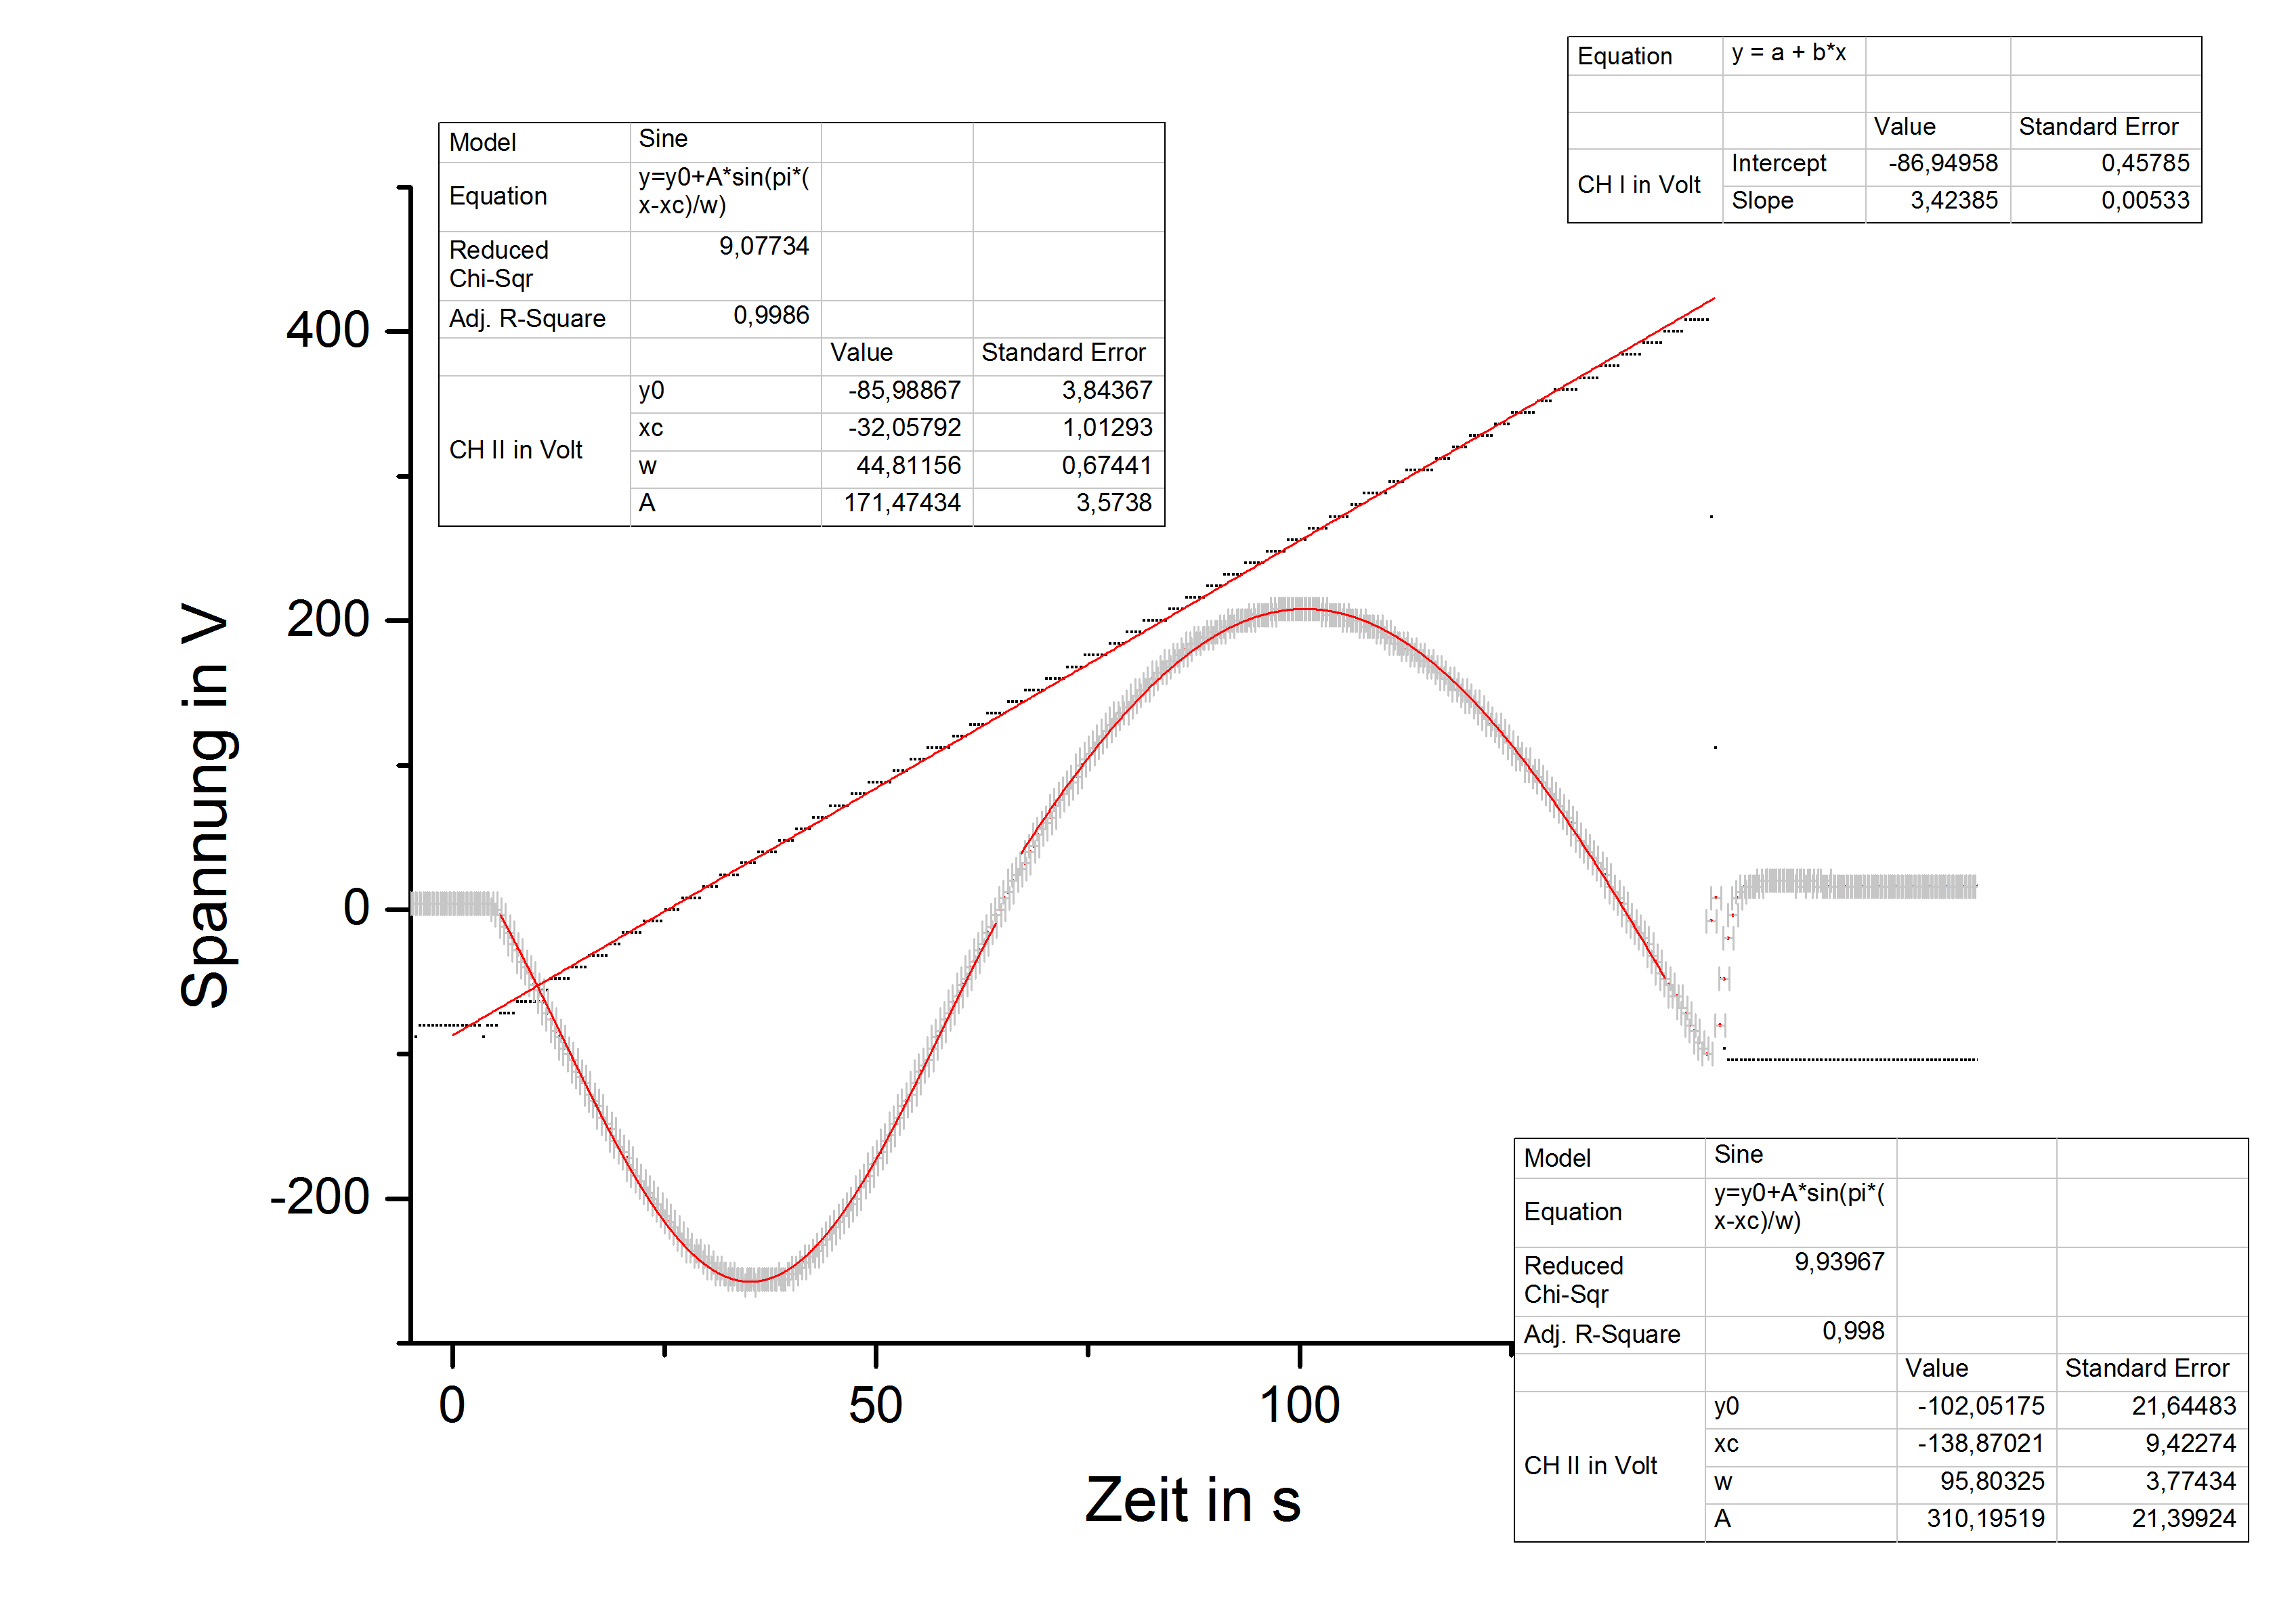
\includegraphics[scale=0.6]{korrigiert.png}
\caption{Durch Sägezahnspannung erzeugtes korrigiertes Signal}
\end{center}
\end{figure}
\clearpage
Damit erhielten wir $k_{tief}=1$ und $k_{hoch}=2$, was zwar zu einer Reduktion des Fehlers führt, jedoch noch immer nicht das bestmögliche Ergebnis darstellt. Wir entschlossen uns dennoch, mit diesem Ergebnis weiterzurechnen, weil wir den Nullpunkt nicht willkürlich verschieben wollten. Somit erhielten wir für die Zeiten, bei denen die Peaks liegen:\\
$x_{tief}=(35,2\pm1,4)s$\\
$x_{hoch}=(101\pm6)s$\\
Nun setzten wir diese Werte jeweils in die Geradengleichung $y=m*x+c$ (s. Diagramm), welche wir für die Sägezahnspannung erhielten, ein. Um die Fehler zu berechnen, verwendeten wir die Gauss'sche Fehlerfortpflanzung:\\
$s_{y}=\sqrt{m^{2}*s_{x}^{2}+s_{c}^{2}+x^{2}*s_{m}^{2}}$\\
Die Differenz der beiden so erhaltenen Spannungen ist:\\
$U=y_{hoch}-y_{tief}=224,2 V$\\
$\Rightarrow s_{U}=\sqrt{s_{y_{tief}}^{2}+s_{y_{hoch}}^{2}}=20,3 V$\\
Da die Fehler allgemein ziemlich groß waren, haben wir die Fehler des Oszilloskops vernachlässigt.\\
Die somit errechnete Spannung entspricht noch nicht zwangsläufig der Spannung $U_{\lambda/2}$, welche wir errechnen sollten. Dies ist der Fall, da das Computerprogramm von einer Dämpfung um den Faktor 100 bei der Sägezahnspannung rechnete und daher die für diese erhaltenen Werte mit demselben Faktor multiplizierte. Um den tatsächlichen Dämpfungsfaktor zu errechnen, verglichen wir am Oszilloskop an unterschiedlichen Kanälen das normale mit dem gedämpften Signal, um Rückschlüsse ziehen zu können. Wir benutzten erneut Sinus-Fits für die Peaks, wie in den folgenden Diagrammen zu sehen ist, welches eines der drei Messreihen darstellt:\\
\begin{figure}[h]
\begin{center}
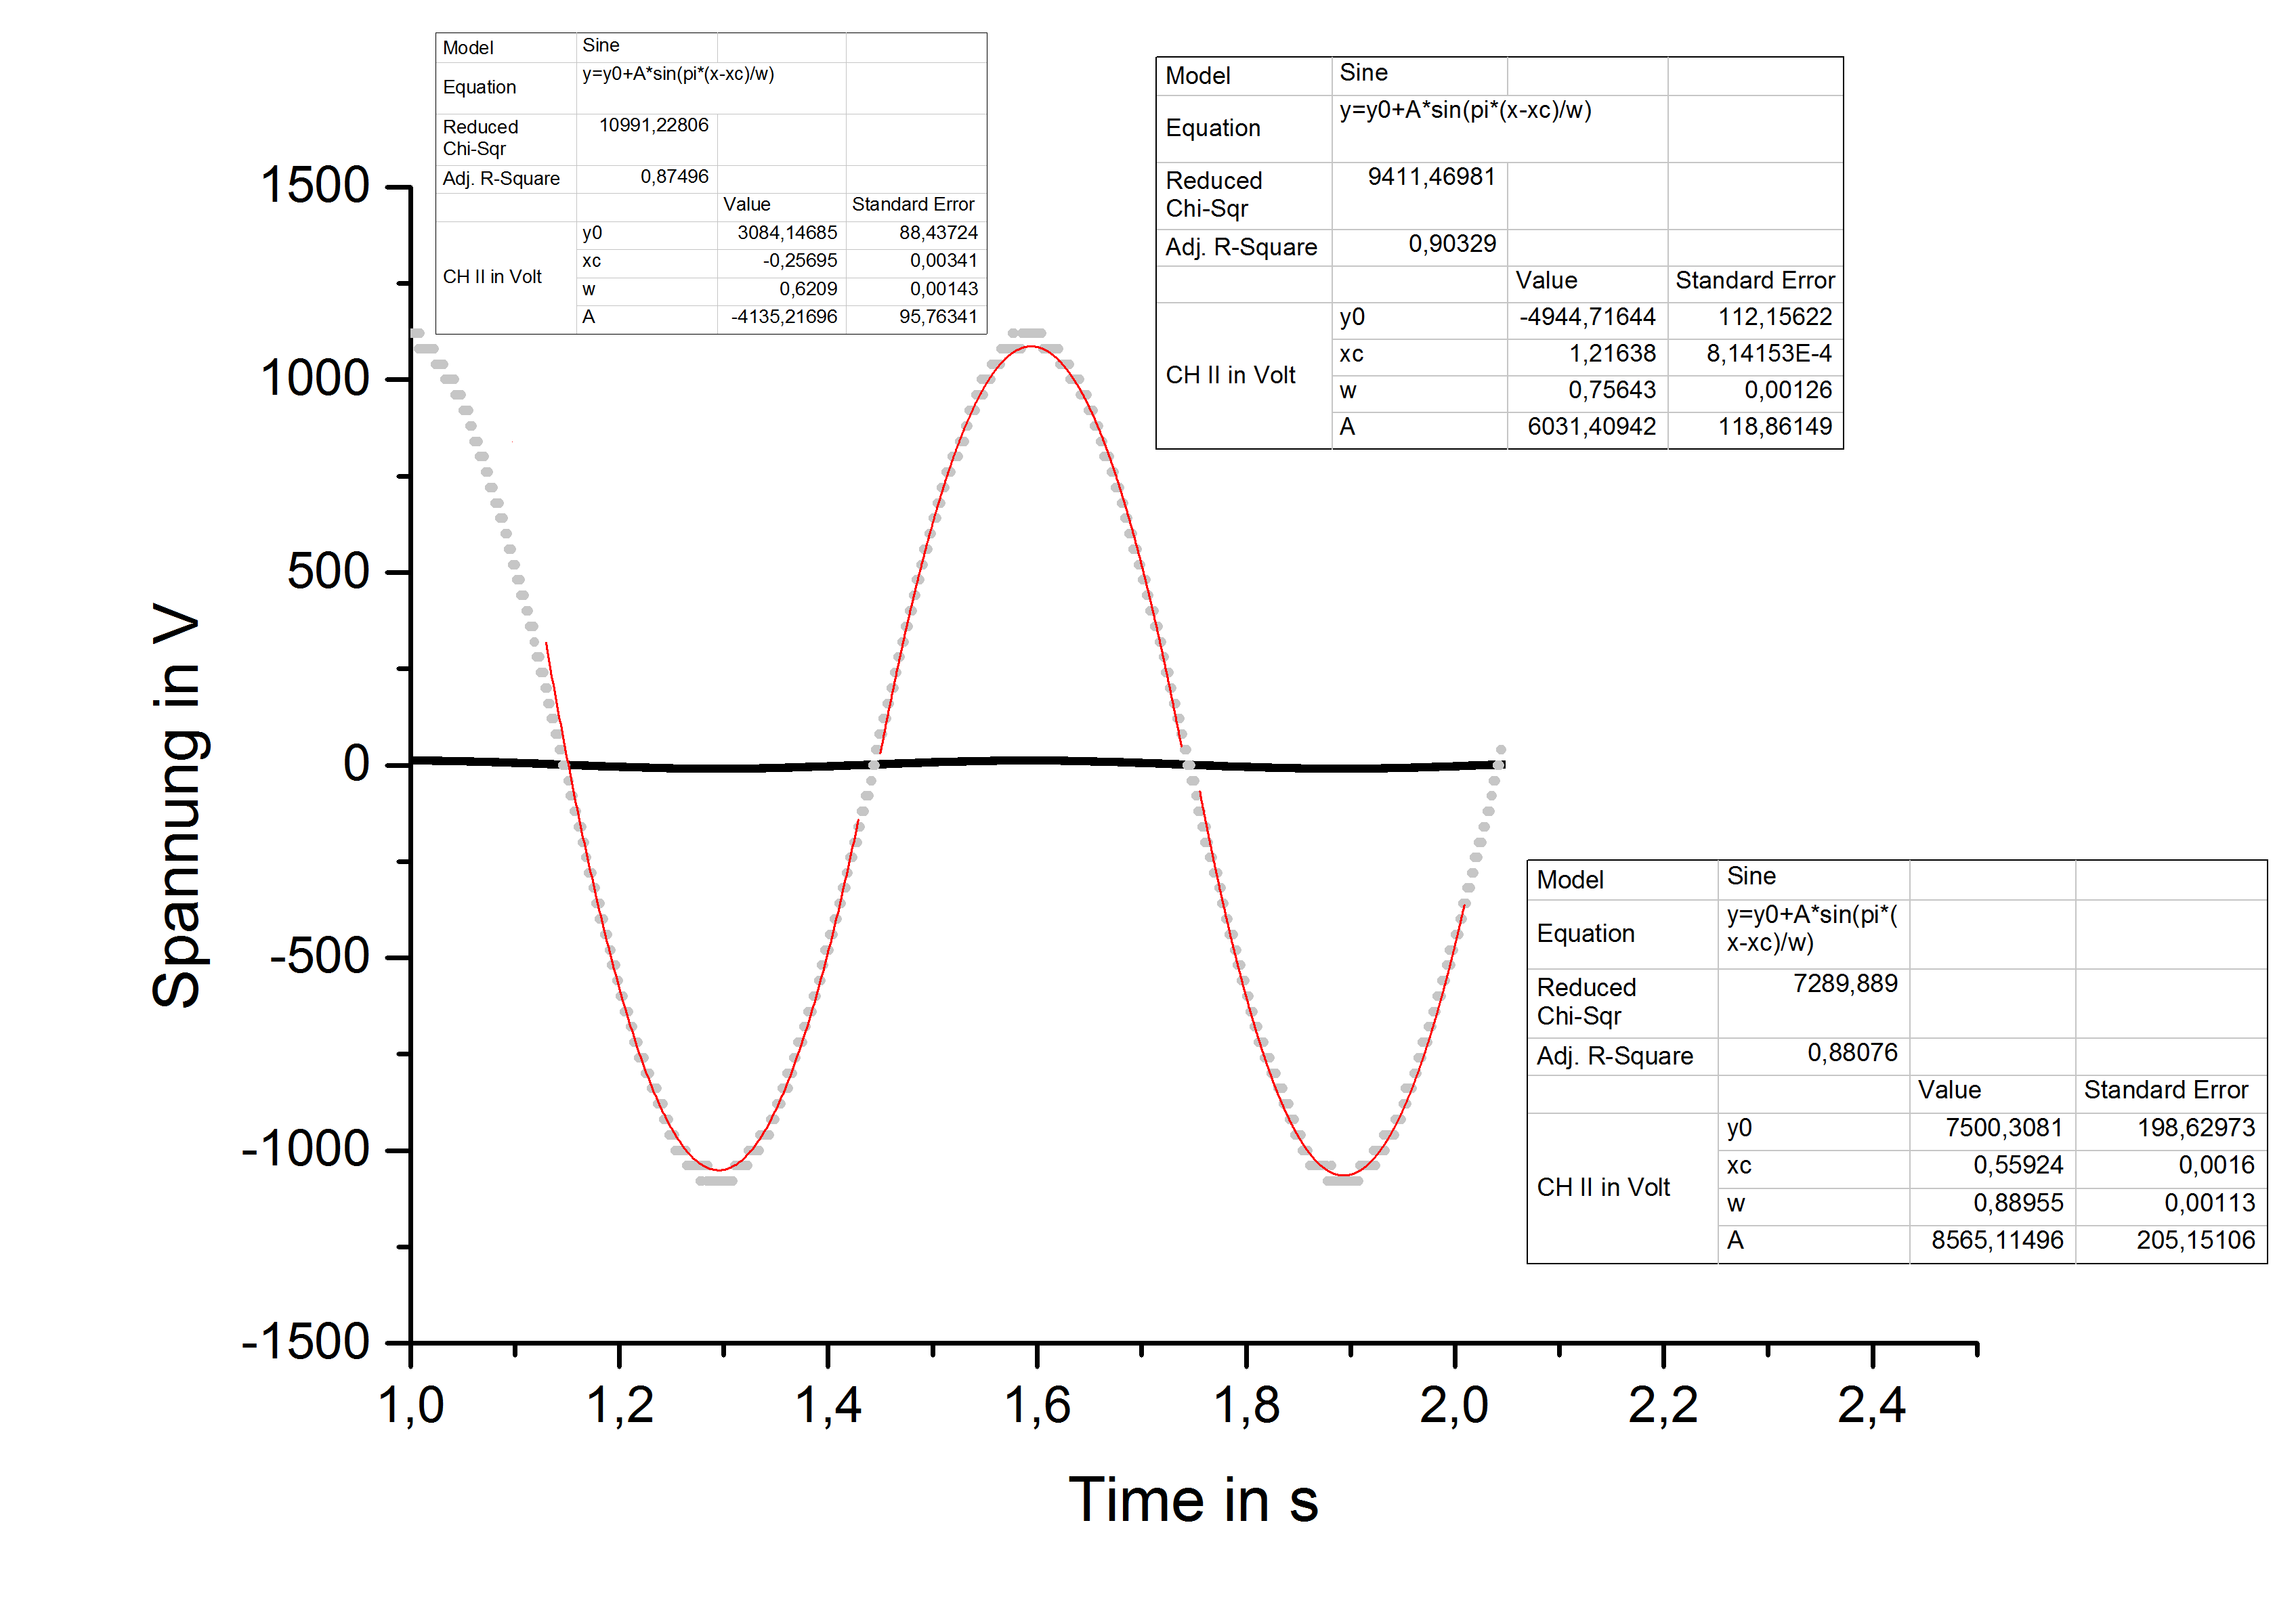
\includegraphics[scale=0.5]{verstaerkt.png}
\caption{Signal ohne Drosselung}
\end{center}
\end{figure}
\clearpage
\begin{figure}[h]
\begin{center}
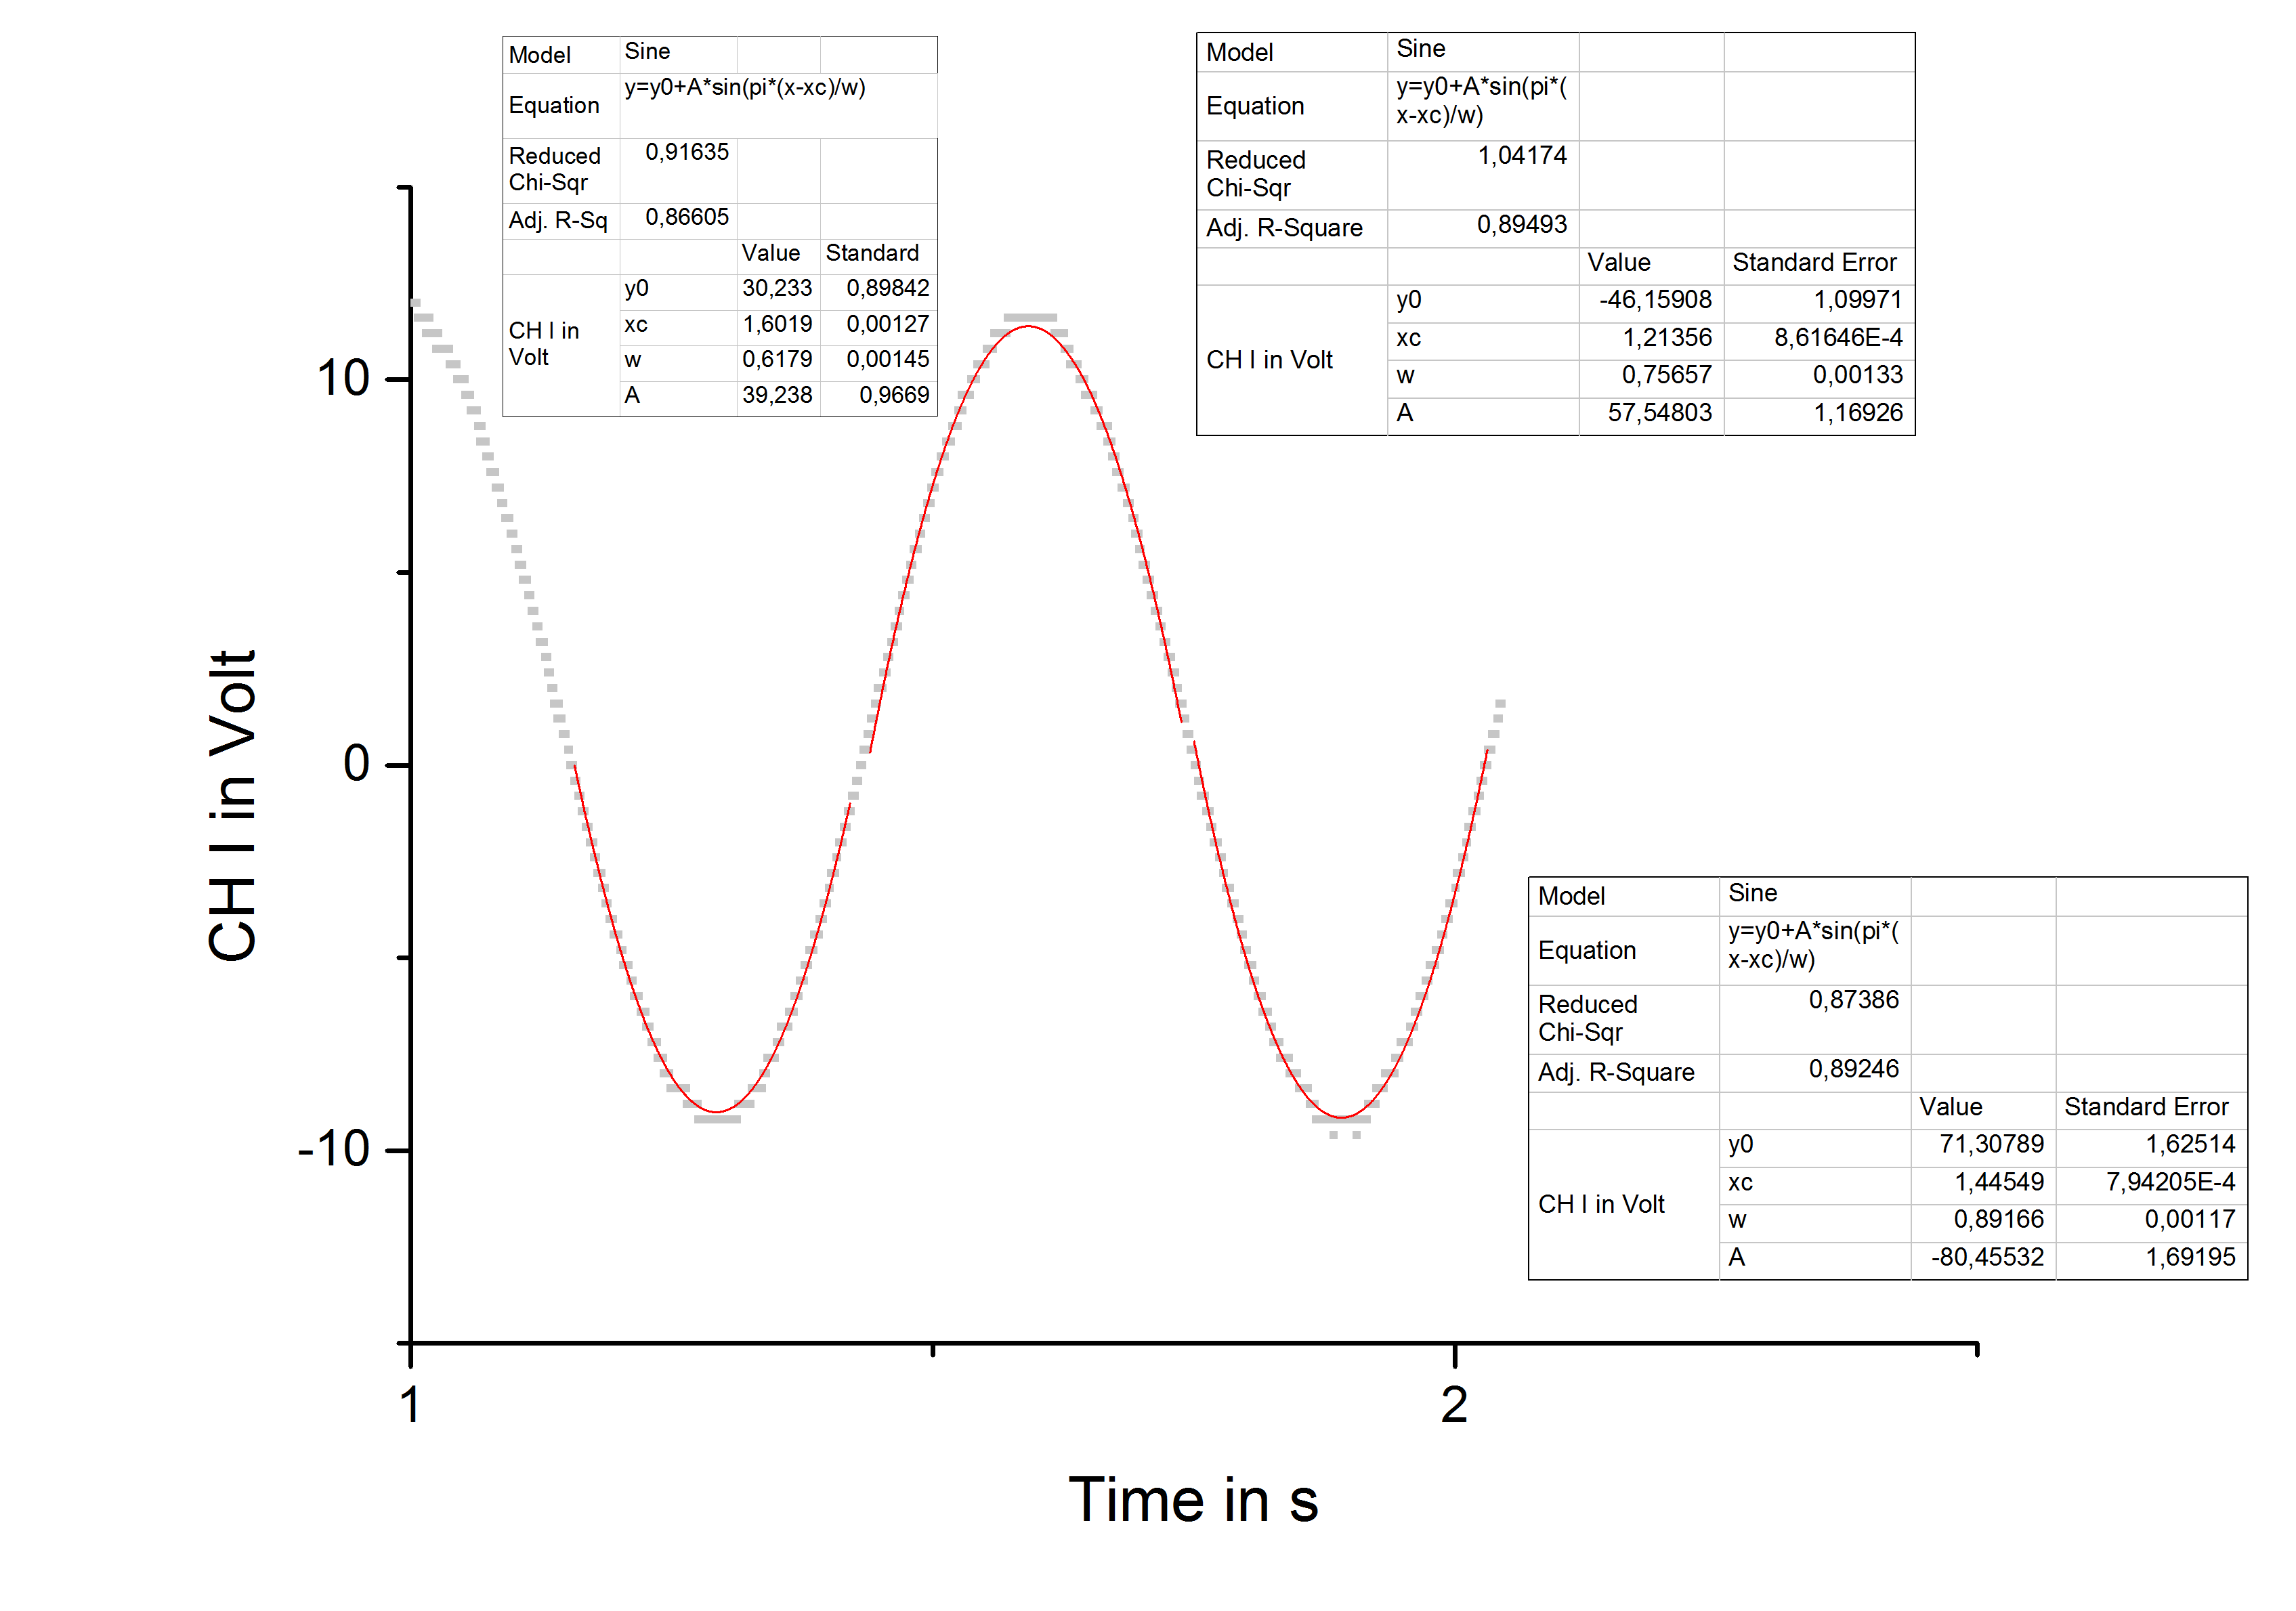
\includegraphics[scale=0.5]{ch1t23.png}
\caption{Gedrosseltes Signal}
\end{center}
\end{figure}
Die tatsächliche Amplitude errechneten wir mit den Formeln $A+y_{0}$ bzw. $y_{0}-A$, je nachdem, wie Origin den Fit erstellte. Für den Fehler gilt: \\
$\Rightarrow s_{Ampl.}=\sqrt{s_{A}^{2}+s_{y_{0}}^{2}}$\\
Für den Faktor, mit welchem die Werte tatsächlich hätten multipliziert werden müssen, gilt somit:\\
\[D=\frac{Ampl_{normal}}{Ampl_{gedrosselt}}\]
\[\Rightarrow s_D=D*\sqrt{(\frac{s_{Ampl_{normal}}}{Ampl_{normal}})^{2}+(\frac{s_{Ampl_{gedrosselt}}}{Ampl_{gedrosselt}})^{2}}\]
Insgesamt erhielten wir 9 Peaks, welche allesamt nach derselben Methode ausgewertet wurden. Für die Verhältnisse der Amplituden gilt:\\
\begin{table}[htbp]
\begin{tabular}{|r|r|r|}
\hline
\multicolumn{1}{|l|}{Peaks} & \multicolumn{1}{l|}{D\_i} & \multicolumn{1}{l|}{s\_D\_i} \\ \hline
1 & 91,4 & 19,6 \\ \hline
2 & 123,8 & 24,0 \\ \hline
3 & 124,6 & 52,1 \\ \hline
4 & 93,3 & 20,6 \\ \hline
5 & 120,7 & 42,7 \\ \hline
6 & 124,1 & 20,5 \\ \hline
7 & 95,4 & 19,7 \\ \hline
8 & 116,4 & 43,2 \\ \hline
9 & 116,7 & 22,4 \\ \hline
\end{tabular}
\end{table}
\clearpage
Da hierbei nur Verhältnisse berechnet wurden, haben wir die Fehler des Oszilloskops vernachlässigt.\\
Um schließlich $\bar{D}$ zu berechnen, verwendeten wir eine gewichtete Mittelung:\\
\[\bar{D}=\sum\limits_{i=1}^{9}\frac{\frac{D_{i}}{\sigma_{i}^{2}}}{\frac{1}{\sigma_{i}^{2}}}\]
Für den Fehler gilt: \\
\[s_{\bar{D}}=\sum\limits_{i=1}^{9}\frac{1}{\frac{1}{\sigma_{i}^{2}}}\]
Somit erhielten wir: \\
$\bar{D}=(107\pm8)$\\
Im Rahmen der Standardabweichung handelt es sich also tatsächlich um eine Verstärkung um den Faktor 100. Um einen genaueren Wert zu erhalten, rechneten wir allerdings:\\
\[U_{\lambda/2}=\frac{\bar{D}}{100}*U\]
Für den Fehler folgt dann mit Gauss'scher Fehlerfortpflanzung:\\
\[s_{U_{\lambda/2}}=\sqrt{(\frac{U_{\lambda/2}}{100})^{2}*s_{\bar{D}}^{2}+(\frac{\bar{D}}{100})^{2}*s_{U_{\lambda/2}}^{2}}\]
Somit erhielten wir:\\
$U_{\lambda/2}=(240\pm30)V$\\
Den elektrooptischen Koeffizienten $r_{41}$ errechneten wir mit der in [Ver] gegebenen Formel (und den dort gegebenen Konstanten):\\
\[r_{41}=\frac{\lambda*d}{4l*U_{\lambda/2}}*\left(\sqrt{0,5*(\frac{1}{n_{1}^{2}}+\frac{1}{n_{3}^{2}})}\right)^{3}=23,4 \frac{pm}{V}\]
Für den Fehler gilt:\\
\[s_{r_{41}}=r_{41}*\frac{s_{U_{\lambda/2}}}{U_{\lambda/2}}=2,8 \frac{pm}{V}\]
Insgesamt gilt also:\\
$r_{41}=(23\pm3)\frac{pm}{V}$\\
Der Literaturwert beträgt $23,4\frac{pm}{V}$. Der mithilfe unserer Messwerte errechnete Wert liegt im Rahmen einer Standardabweichung auf dem Literaturwert. 
\subsubsection{Sinusmodulierte Gleichspannungsmethode}
Bei dieser Messreihe wurde an die von einer Gleichspannung überlagerte Sinusspannung an die Pockelszelle angelegt. Wir veränderten den Gleichspannungsanteil, bis eine Verdopplung der Frequenz am Oszilloskop sichtbar war. Diese Spannung notierten wir. Wir taten dies für negative wie für positive Spannungen jeweils 10-mal (für die Messreihe s. Anhang). Somit errechneten wir $U_{\lambda/2}$ folgendermaßen:\\
\[\overline{U_{pos}}=\frac{1}{10}\sum\limits_{i=1}^{10}U_{pos_{i}}\]
Der Fehler errechnete sich als reiner statistischer Fehler, da uns für das Gerät kein Fehler der Anzeige bekannt war, weshalb wir diesen vernachlässigten (wodurch die Fehler zu klein sind):\\
\[s_{\overline{U_{pos}}}=\sqrt{\frac{1}{9}\cdot\sum\limits_{i=1}^{10}\left(U_{pos_{i}}-\overline{U_{pos}}\right)^{2}}\]
Für die negativen Spannungen wurden die Werte analog berechnet. Somit erhielten wir:\\
$\overline{U_{pos}}=(129,4\pm0,2)V$\\
$\overline{U_{neg}}=(-121,8\pm0,4)V$\\
Für $U_{\lambda/2}$ gilt somit:\\
\[U_{\lambda/2}=\overline{U_{pos}}-\overline{U_{neg}}=251,2 V\] und für den Fehler: \[s_{U_{\lambda/2}}=\sqrt{s_{\overline{U_{pos}}}^{2}+s_{\overline{U_{neg}}}^{2}}=0,5 V\]
Analog zum vorherigen Kapitel errechneten wir damit den elektrooptischen Koeffizienten und erhielten:\\
$r_{41}=(22,41\pm0,04)\frac{pm}{V}$
Der Fehler ist, wie bereits erwähnt, zu klein. Dennoch ist auch zu beobachten, dass der Wert selbst nicht so genau ist wie der mithilfe der Sägezahnmethode bestimmte. Dies könnte auf einen systematischen Fehler hinweisen, beispielsweise durch eine nicht vorgesehene Erwärmung der Kristalle, was die natürliche Doppelbrechung beeinflussen kann.




\subsection{Faraday-Effekt}
\subsubsection*{Bestimmung der Verdetkonstante}
Um die Verdetkonstante zu berechnen, haben wir die Rotation des Lichtes welches durch ein Schwerflintglas in einer Spule verlief, in Abhängigkeit des Magnetfelds der Spule gemessen.
\begin{figure}[h]
\begin{center}
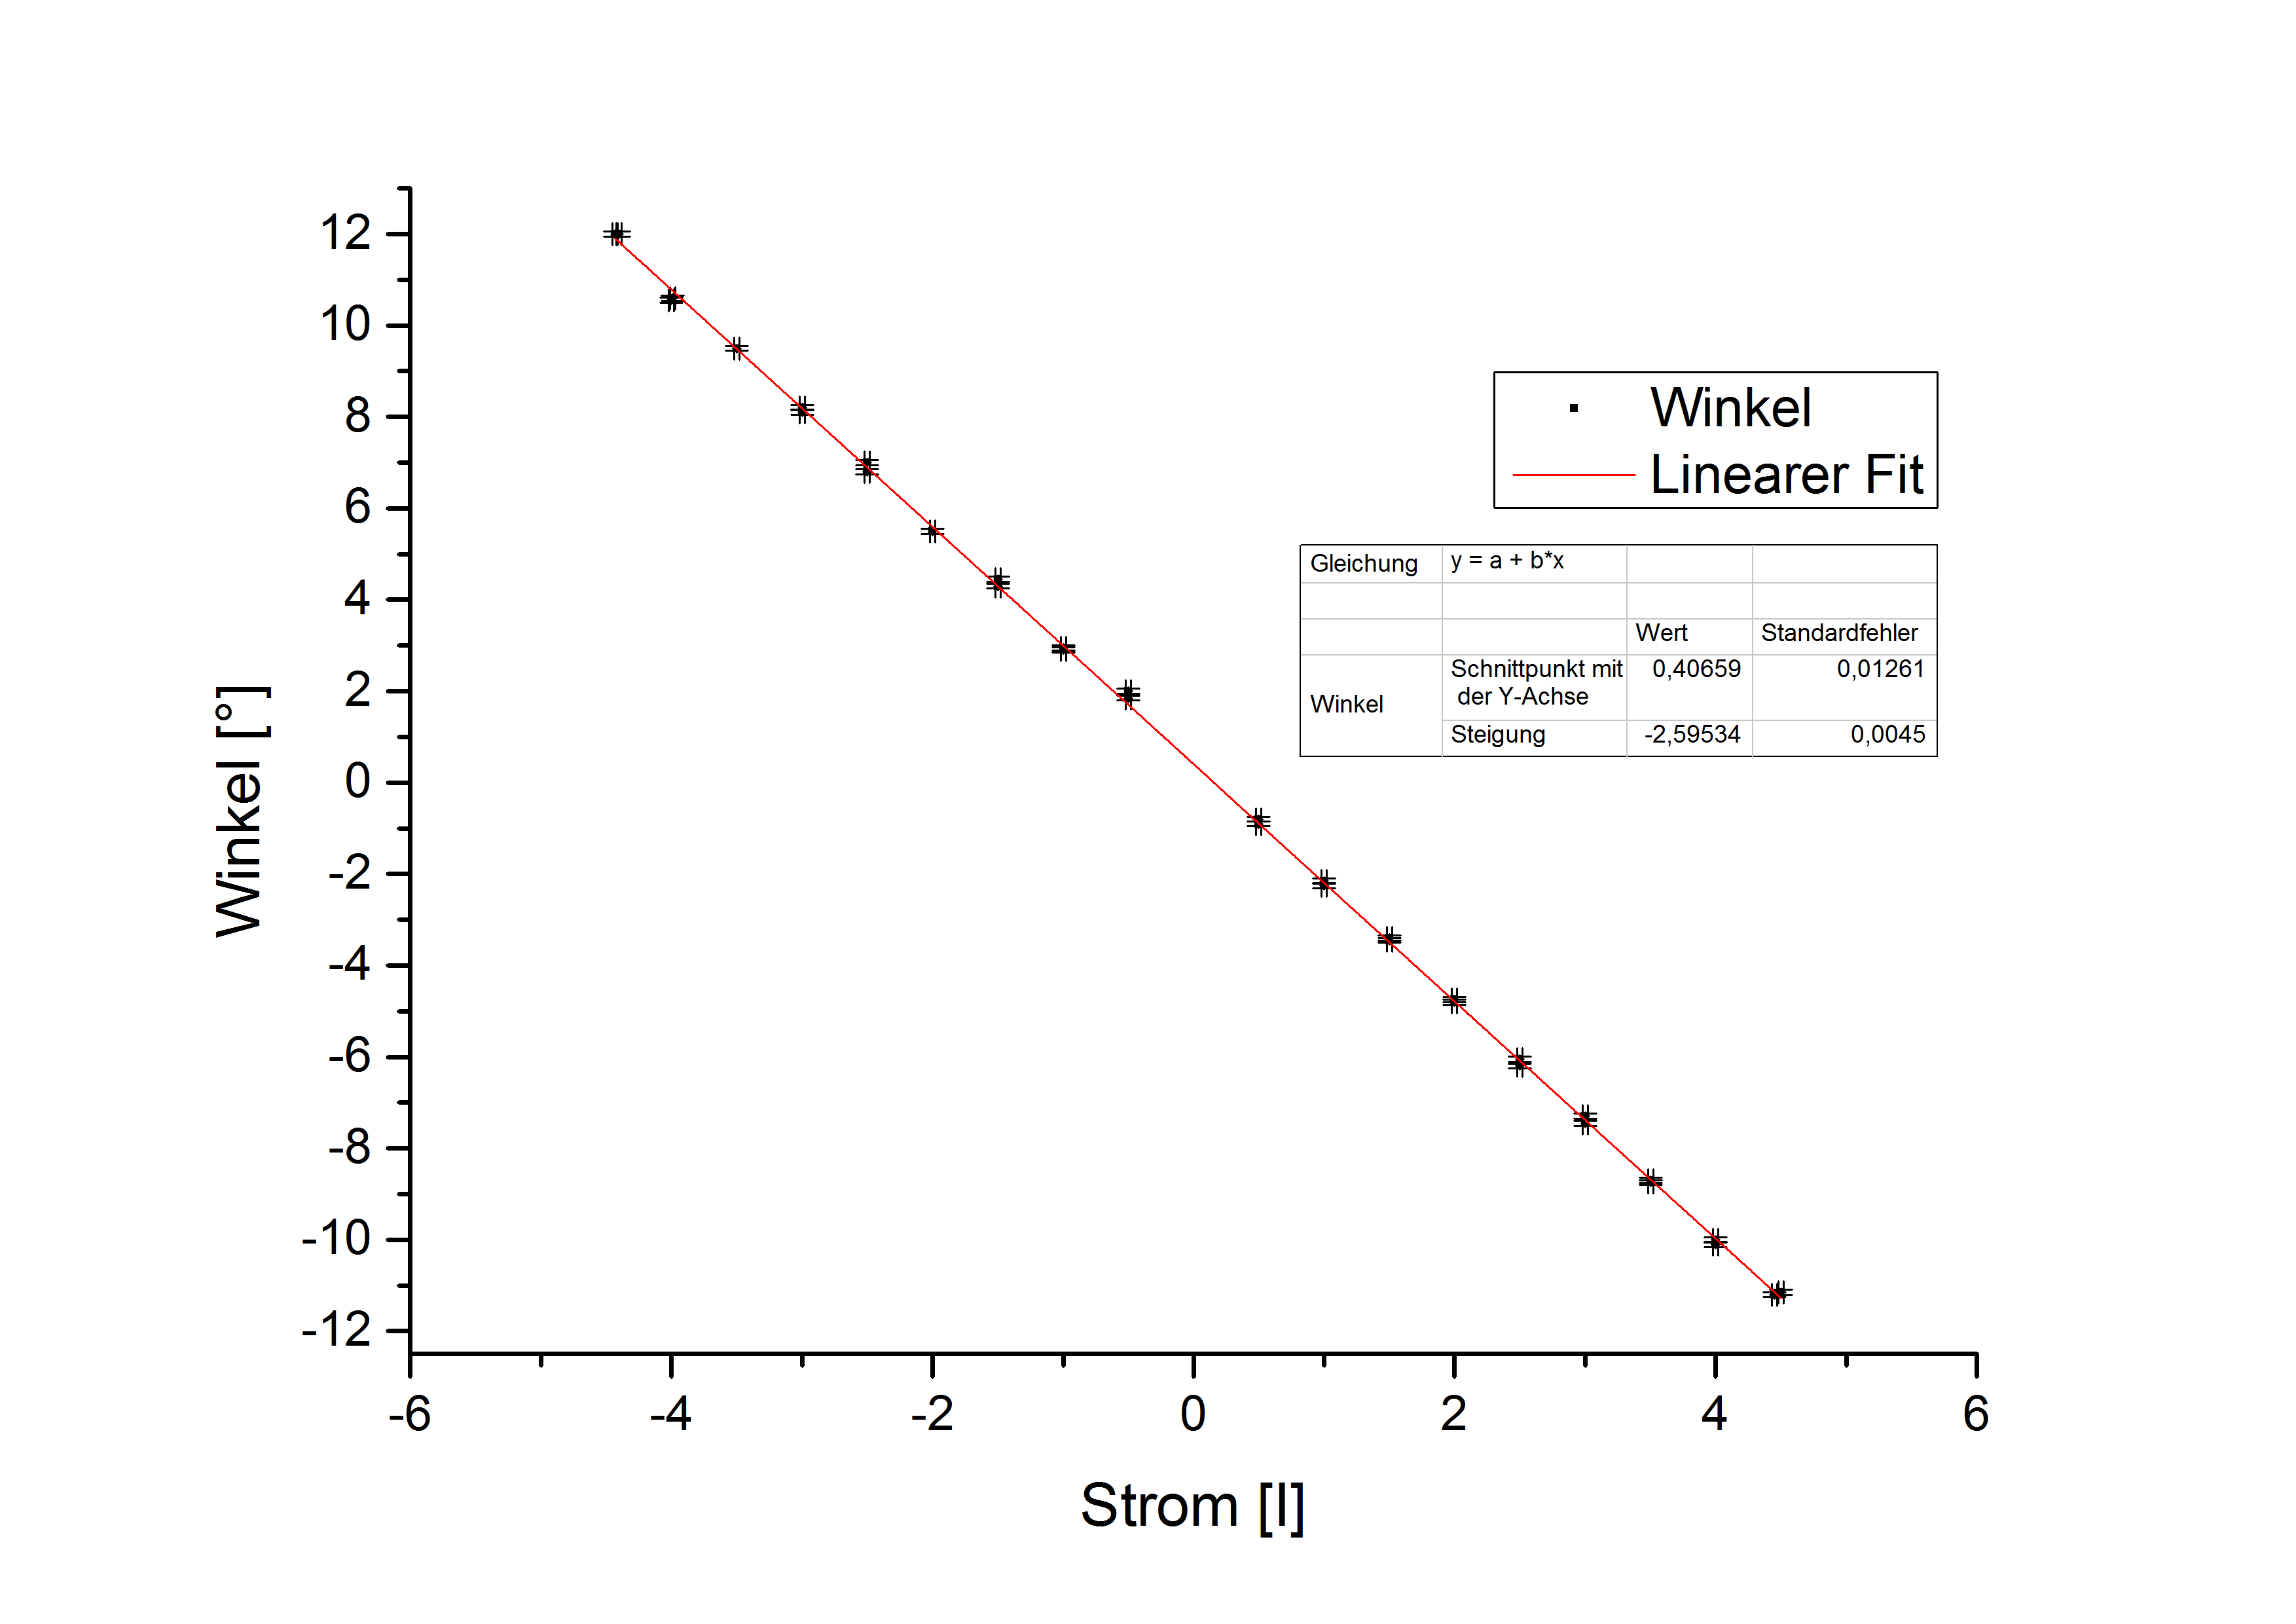
\includegraphics[scale=0.3]{faraday_lin}
\caption{Linearer Fit beim auftragen von Winkel über Stromstärke}
\label{fig:faraday_lin}
\end{center}
\end{figure}
~\\
Die Ableseungenauigkeit auf die Winkel haben wir durch eine gesonderte Messung zu beginn des Versuches bestimmt, siehe Anhang. Hierbei haben wir bei der selben Spannung Mehrfach den Winkel abgelesen, bei denen das Halbschattenpolarimeter innen und außen die selbe Intensität aufweist. Da der korrekte Winkel nicht vorlag können wir keine Personenbezogene Wichtung vornehmen. Als Fehler auf die Messung des Winkels in den weiteren Versuchsteilen haben wir, dadurch die Standardabweichung der Einzelwerte benutzt, diese beträgt $s_\alpha = 0,06\,^{\circ} $.\\
Um das Verhältnis von Stromstärke $I$ und der magnetischen Feldstärke $H$ der Spule zu erhalten benutzen wir das Biot-Savart-Gesetz. Die Herleitung und Berechnung der magnetischen Feldstärke kann in der Arbeit von Bernd Herrman ("Elektrooptischer Effekt und Faraday Effekt") nachgeschlagen werden.
\begin{center}
\[ d\alpha = V \cdot H(z)\cdot dz  \Rightarrow \alpha = 2556 \cdot V \cdot I\]
\[ V = \frac{\alpha}{2556 \cdot I}\]
\end{center}
Hierbei ist $\alpha$ der Winkel um welches sich dir Polarität gedreht hat, $V$ ist die Verdetkonstante und $I$ die Stromstärke. Aus dem linearen Fit oben lässt sich die Steigung $b$ auslesen. Diese entspricht genau dem Verhältnis aus:
\[b = \frac{Winkel}{Stromstärke}=\frac{\alpha}{I}\]
\[\Rightarrow V=\frac{b}{2556}\]
Wenn wir nun von Grad-maß zu Radiant wechseln erhalten wir:
\begin{center}
\[V=b \cdot \frac{3979}{213} \cdot 10^{-3} \frac{min}{Oe ~ cm} \]
\end{center}
Der Fehler auf $V$ ergibt sich aus:
\begin{center}
\[s_{V}= V \cdot \frac{s_b}{b}\]
\end{center}
Die Verdetkonstante für Schwerflintglas und die Wellenlänge des Lichtes der Natriumdampflampe von $\lambda = 589 nm$, beträgt:
\begin{center}
\[ V_{SF,589}=(-0,04848\pm0,00008) \frac{Min}{Oe~cm} \]
\end{center}

~\\
\subsubsection*{$2 \epsilon$ Messung}
Nun haben wir zum vermessen des Winkels $\beta$ um welchen die Polarisationsrichtungen des Halbschattenpolarimeters verschoben sind, jeweils den Winkel der beiden Hälften vermessen bei denen sie jeweils am dunkelsten sind. Die Messwerte hierfür befinden sich im Anhang. Aus den zwei Werten wurde jeweils der Mittelwert berechnet.\\
Man erhält also:\\
\[ \alpha_{1,J}=9,15\,^{\circ} ,~~~~~~~~~~~ \alpha_{1,D}=8,10\,^{\circ} \]
\[ \Rightarrow \alpha_1 = (8,63\pm0,04)\,^{\circ} \]
\[ \alpha_{2,J}=171,4\,^{\circ} ,~~~~~~~~~~~ \alpha_{2,D}=175,4\,^{\circ} \]
\[ \Rightarrow \alpha_1 = (173,4\pm0,04)\,^{\circ} .\]
Der Fehler folgt aus der oben genannten Fehlermessung.
Für die $2\epsilon$ Messung gilt nun:
\[ 2\epsilon = \mid \alpha_1 - \alpha_2 \mid = (164,77\pm0,06)\,^{\circ} \]
Der Fehler berechnet sich aus $s_{2\epsilon}=\sqrt{2} \cdot s_{\alpha_1}$, da die beiden Fehler auch hier als gleich angenommen werden müssen.\\
Die großen Unterschiede der obigen $2\epsilon$-Messung könnte daran liegen, dass einer von uns oder beide die zu vermessende Stelle nicht richtig getroffen hat. Da wir auch hier keinen Literatur-/Eichwerte kennen, sind die Messergebnisse gleich gewichtet. Da wir wissen, dass die Maximalstellen mit bloßem Auge schlecht zu bestimmen sind liegt es nahe, dass der statistische Fehler hier zu klein ist.
\clearpage
\section{Zusammenfassung}
\subsection{Pockels-Effekt}
In diesem Teil des Versuchs bestimmten wir den elektrooptischen Koeffizienten $r_{41}$ von ADP mithilfe des Pockels-Effekts. Alle hierfür benötigten Werte sind in der Versuchsanleitung gegeben, nur die Halbwellenspannung $U_{\lambda/2}$ musste noch bestimmt werden. Wir taten dies mit zwei unterschiedlichen Methoden und erhielten folgende Werte:\\
\begin{center}
$r_{41_{Sägezahn}}=(23\pm3)\frac{pm}{V}$\\
$r_{41_{Sinus}}=(22,41\pm0,04)\frac{pm}{V}$\\
\end{center}
Der Literaturwert beträgt:\\
$r_{41_{Lit}}=23,4\frac{pm}{V}$ (Quelle: [Ver])
Der mithilfe der Sägezahnmethode bestimmte Wert stimmt im Rahmen einer Standardabweichung mit dem Literaturwert überein. Der mithilfe der Sinusmethode bestimmte Wert ist zwar in der Größenordnung recht nahe am Literaturwert, allerdings ist der Fehler sehr klein. Eine detaillierte Diskussion wurde im Unterkapitel "Pockels-Effekt/Linearer elektrooptischer Effekt" der Auswertung vorgenommen.\\
\subsection{Faraday-Effekt}
Wir nutzten den Faraday-Effekt, um die Verdet-Konstante von Schwerflintglas zu bestimmen. Dabei erhielten wir:\\
\begin{center}
$V=(-0,04848\pm0,00008)\frac{Min}{Oe*cm}$\\
\end{center}
Die Herstellerangabe lautet $V=-0,05 \frac{Min}{Oe*cm}$. Wie man sieht, ist in der Größenordnung der Wert nahe an dieser, allerdings ist der Fehler sehr klein. Eine Diskussion dieses Sachverhalts ist im Unterkapitel "Faraday-Effekt/Magnetooptischer Effekt" der Auswertung zu finden.\\
Für den Winkel zwischen den Polarisationsebenen erhielten wir $2\epsilon=(164,77\pm0,05)\,^\circ $
\clearpage
\section{\textsc{Quellenverzeichnis}}

[hep]: Teilchenwelt, Universität Freiburg, Prof. Dr. Herten http://hep.uni-freiburg.de/Kamiokanne/PM.png \\
~[ung]: Universität Göttingen, http://lp.uni-goettingen.de/get/bigimage/1561\\
~[ver]: Versuchsanleitung, Fortgeschritten Praktikum, Physikalisches Institut, Albert-Ludwig-Universität Freiburg\\
~[REB]: R.E. Bell: "Coincide Techniques and the Measurement of Short Mean Lives", S.914
\subsection{Sourcecode zu Abbildung~\ref{fig:stm2}}
\begin{minted}[mathescape,
               linenos,
               numbersep=10pt,
               gobble=0,
               frame=lines,
               framesep=2mm]{python}
from scipy.fftpack import fft
import numpy as np
import matplotlib.pyplot as plt
# Number of samplepoints
N = 600
# sample spacing
T = 1.0 / 800.0
x = np.linspace(0.0, N*T, N)
y = np.sin(50.0 * 2.0*np.pi*x) + 0.5*np.sin(80.0 * 2.0*np.pi*x)
yf = fft(y)
xf = np.linspace(0.0, 1.0/(2.0*T), N/2)
from scipy.signal import blackman
w = blackman(N)
ywf = fft(y*w)

f, a = plt.subplots(1, 2, figsize = (10,5))
a[0].plot(xf, 2.0/N * np.abs(yf[0:N/2]))
a[0].plot(xf, 2.0/N * np.abs(ywf[0:N/2]))
a[0].grid(True)
a[0].legend(['FFT', 'FFT mit window'])
a[0].set_xlabel("Frequenz $k$")
a[0].set_ylabel("Leistungsspektrum $2|F(k)|/N$")
a[1].semilogy(xf[1:N/2], 2.0/N * np.abs(yf[1:N/2]) )
a[1].semilogy(xf[1:N/2], 2.0/N * np.abs(ywf[1:N/2]) )
a[1].set_xlabel("Frequenz $k$")
a[1].legend(['FFT', 'FFT mit window'])
a[1].grid(True)

plt.savefig("/home/vsilv/Programming/uni/physik/fp/RTM_03.09/pics/stm2.pdf")
plt.show()
\end{minted}
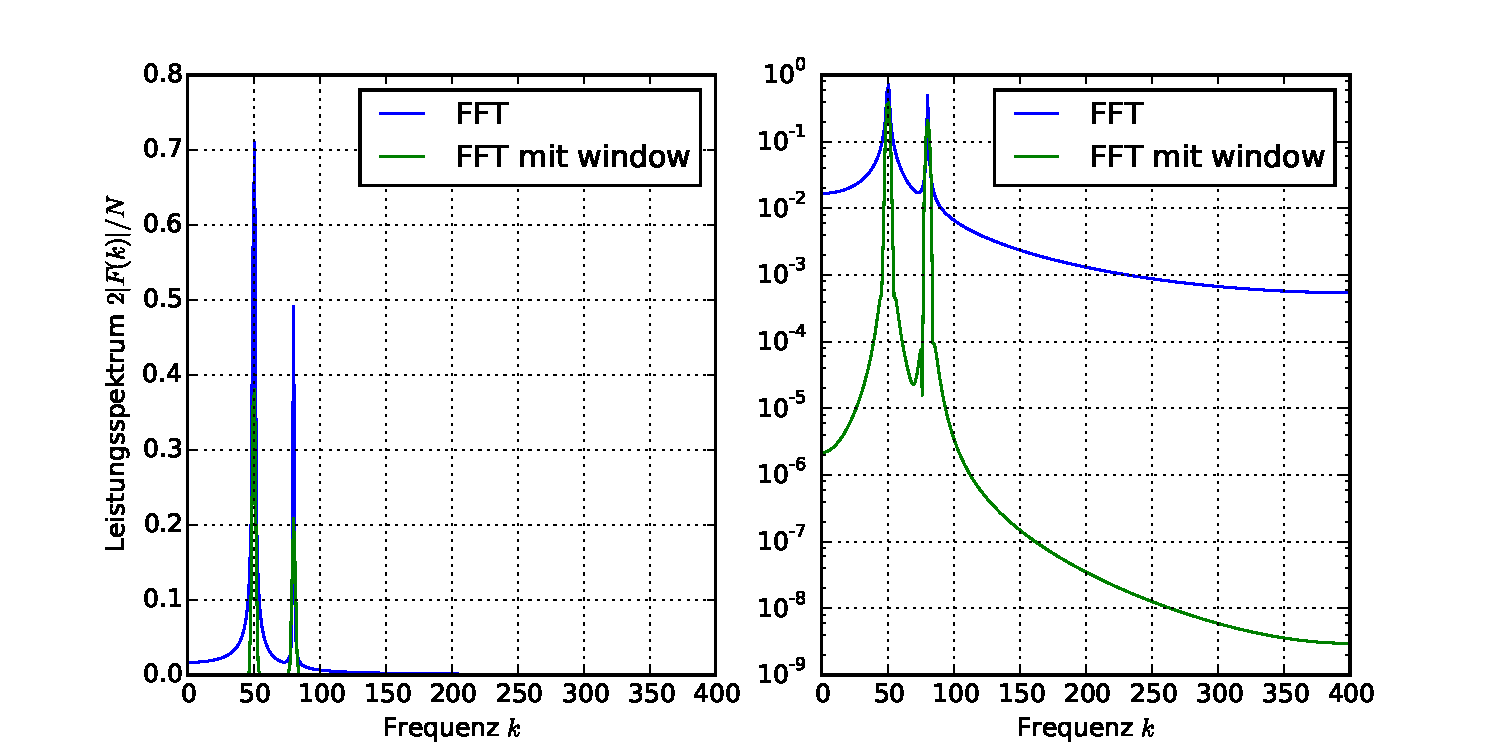
\includegraphics[width=17cm]{pics/stm2}




%Inhaltsverzeichnis
\end{document}
